\documentclass{article}
\usepackage[letterpaper, margin = 1 in]{geometry}
\usepackage{graphicx}
\graphicspath{.}
\usepackage{float}
\usepackage{caption}
\usepackage{subcaption}


\begin{document}

\noindent \textbf{Flat Plate} \\ \\
\noindent \textbf{Unsteady Lift}\\ \\
Vortex of strength $\Gamma$ = -0.02 started upstream at (-4.5,0.04). Graph below shows comparison of obtained results to the analytical lift response of a flat plate to a passing vortex. Note that the lift for both analytical and numerical results have been `normalized' by the strength of the vortex $\Gamma$.\\
\begin{equation}
L = \rho \Gamma \frac{c}{2} e^{-kh} \big(-i S\big(k \big) \big)
\end{equation}

\begin{figure}[h]
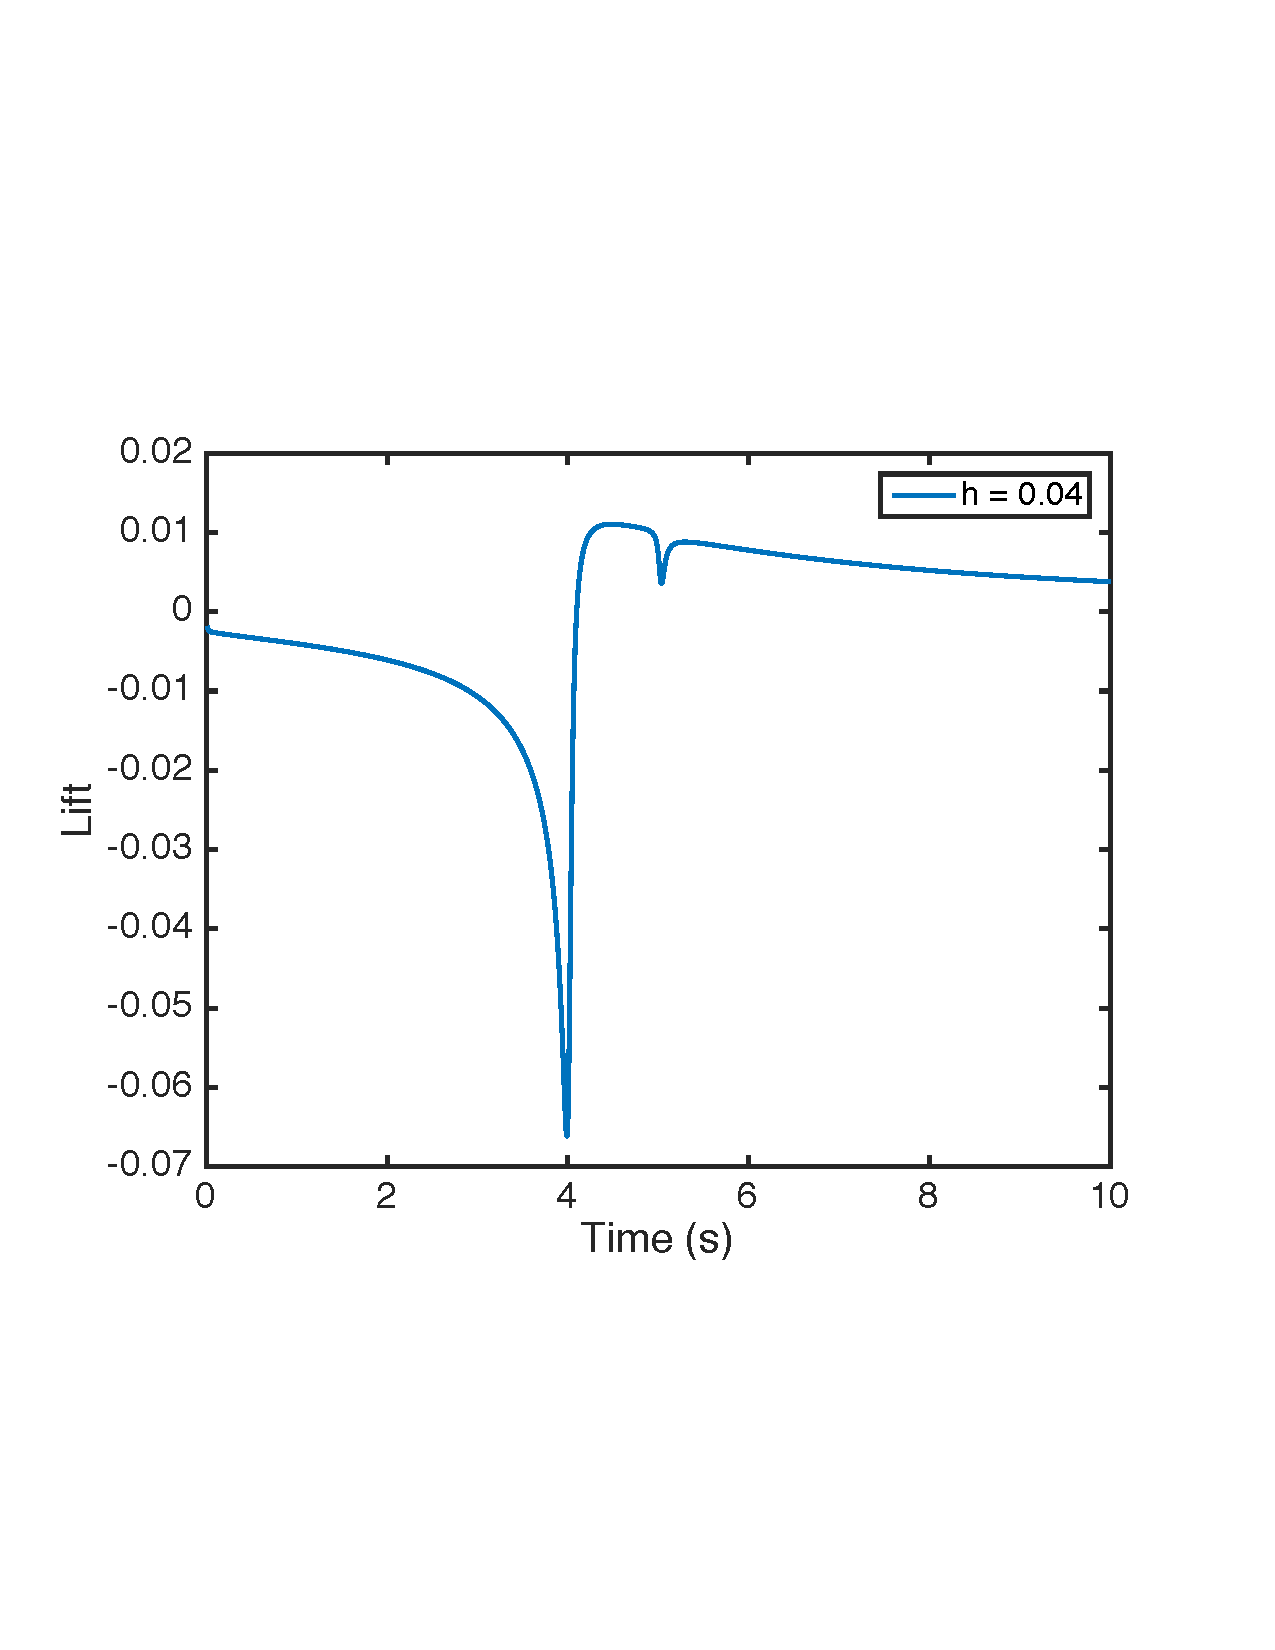
\includegraphics[width = 4 in, height = 3 in]{Lift_Curve}
\centering
\caption{Lift Curve Response of Flat Plate to Passing Vortex}
\end{figure}

\begin{figure}[h]
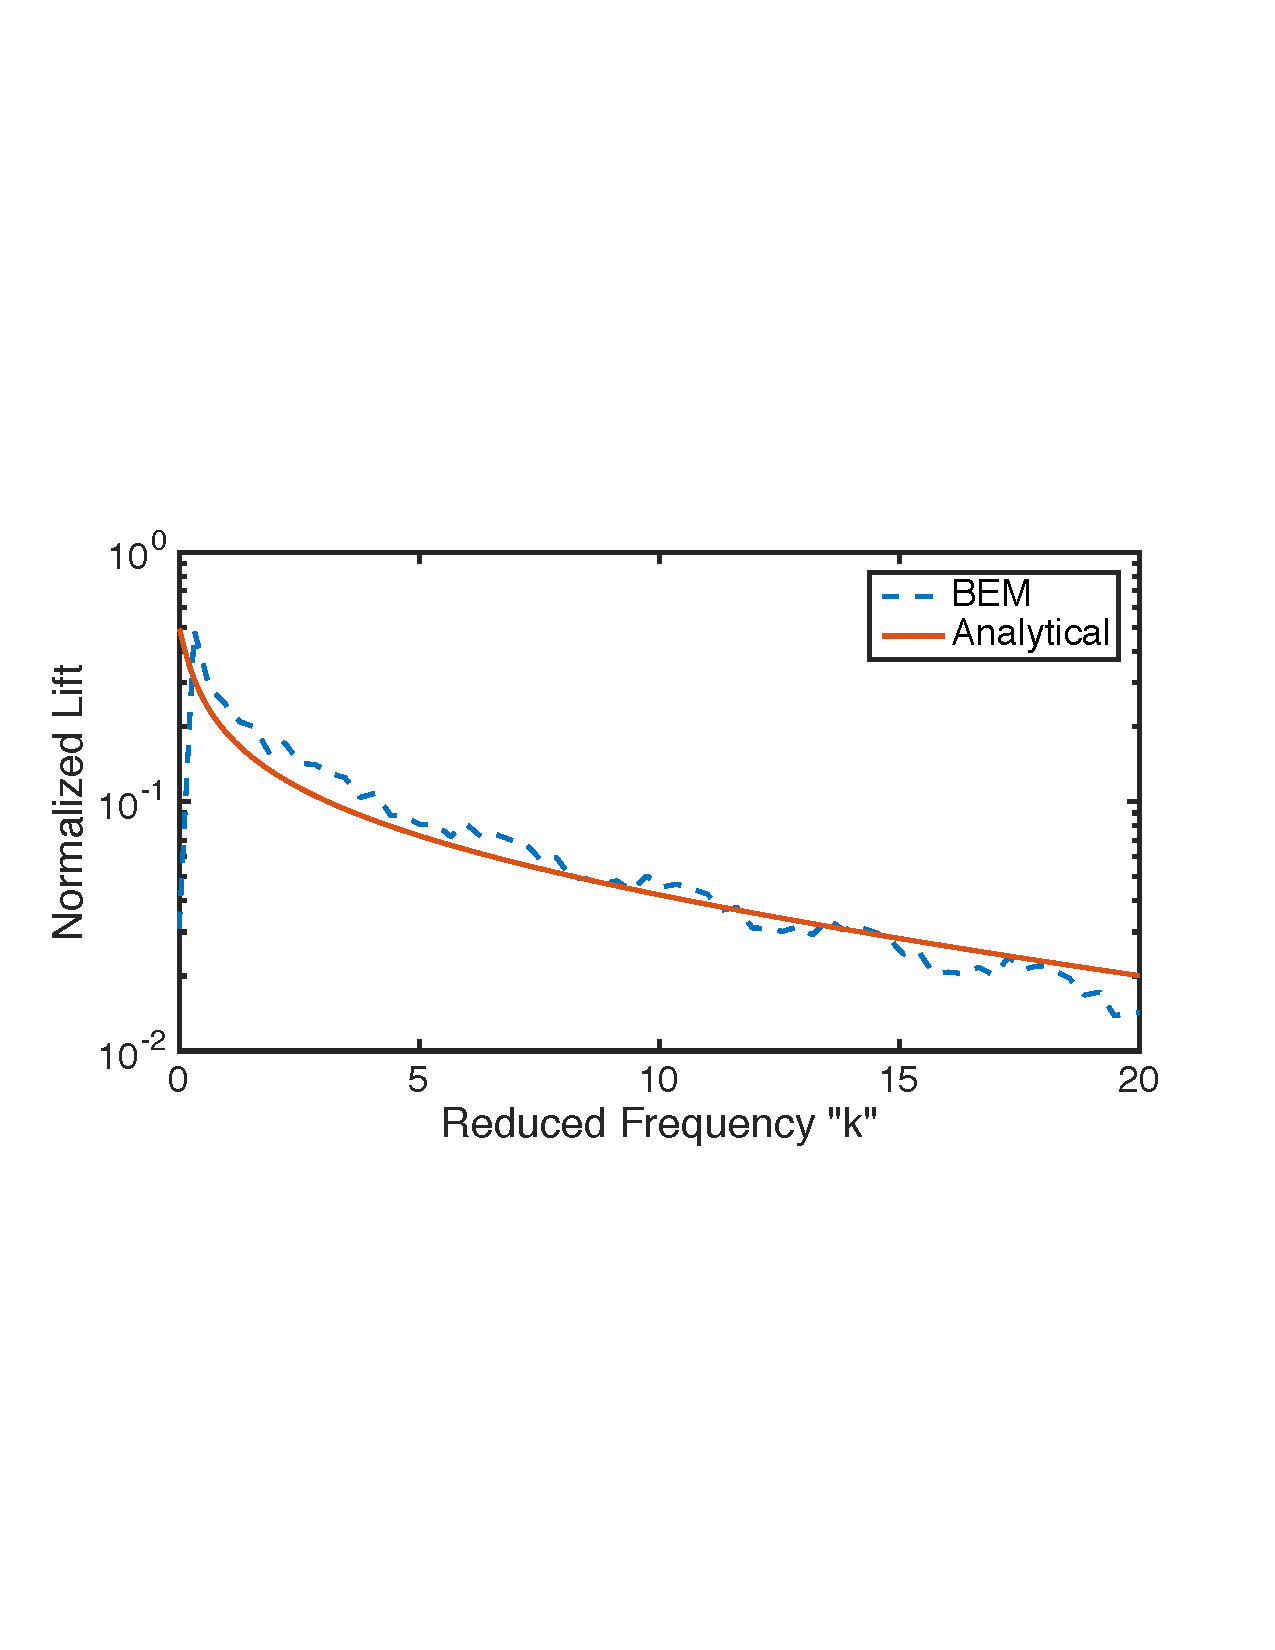
\includegraphics[width = 4 in, height = 3 in]{SearsVsBEM}
\centering
\caption{Analytical and BEM Spectrum of Lift for Vortex Passing Flat Plate}
\end{figure}
\newpage


\noindent For further validation purposes, the BVI results obtained from the Boundary Element method code was compared to other previously validated codes. The figure below shows the BEM results compared to Possio, an asymptotic method, and a method by Ayton. Also overlayed on the plot is the analytical Sears lift for the BVI problem. \\ \\
The asymptotic method, possio, and real AF method developed by Ayton are all gust problem approaches which require the user to input the mach numbers, angle of attack and spectral decompositions of the gust being studied. In the case of the BVI code, the height of passage of the imposed vortex becomes and important parameter. At higher frequencies, it is known that the lift scales as $exp(-kh)$ where h is the minimum passing distance of the vortex over the mean camber line of the airfoil. In order to obtain comparable results to the gust problem, this factor was removed from the obtained results and both lifts were appropriately normalized.

\begin{figure}[h]
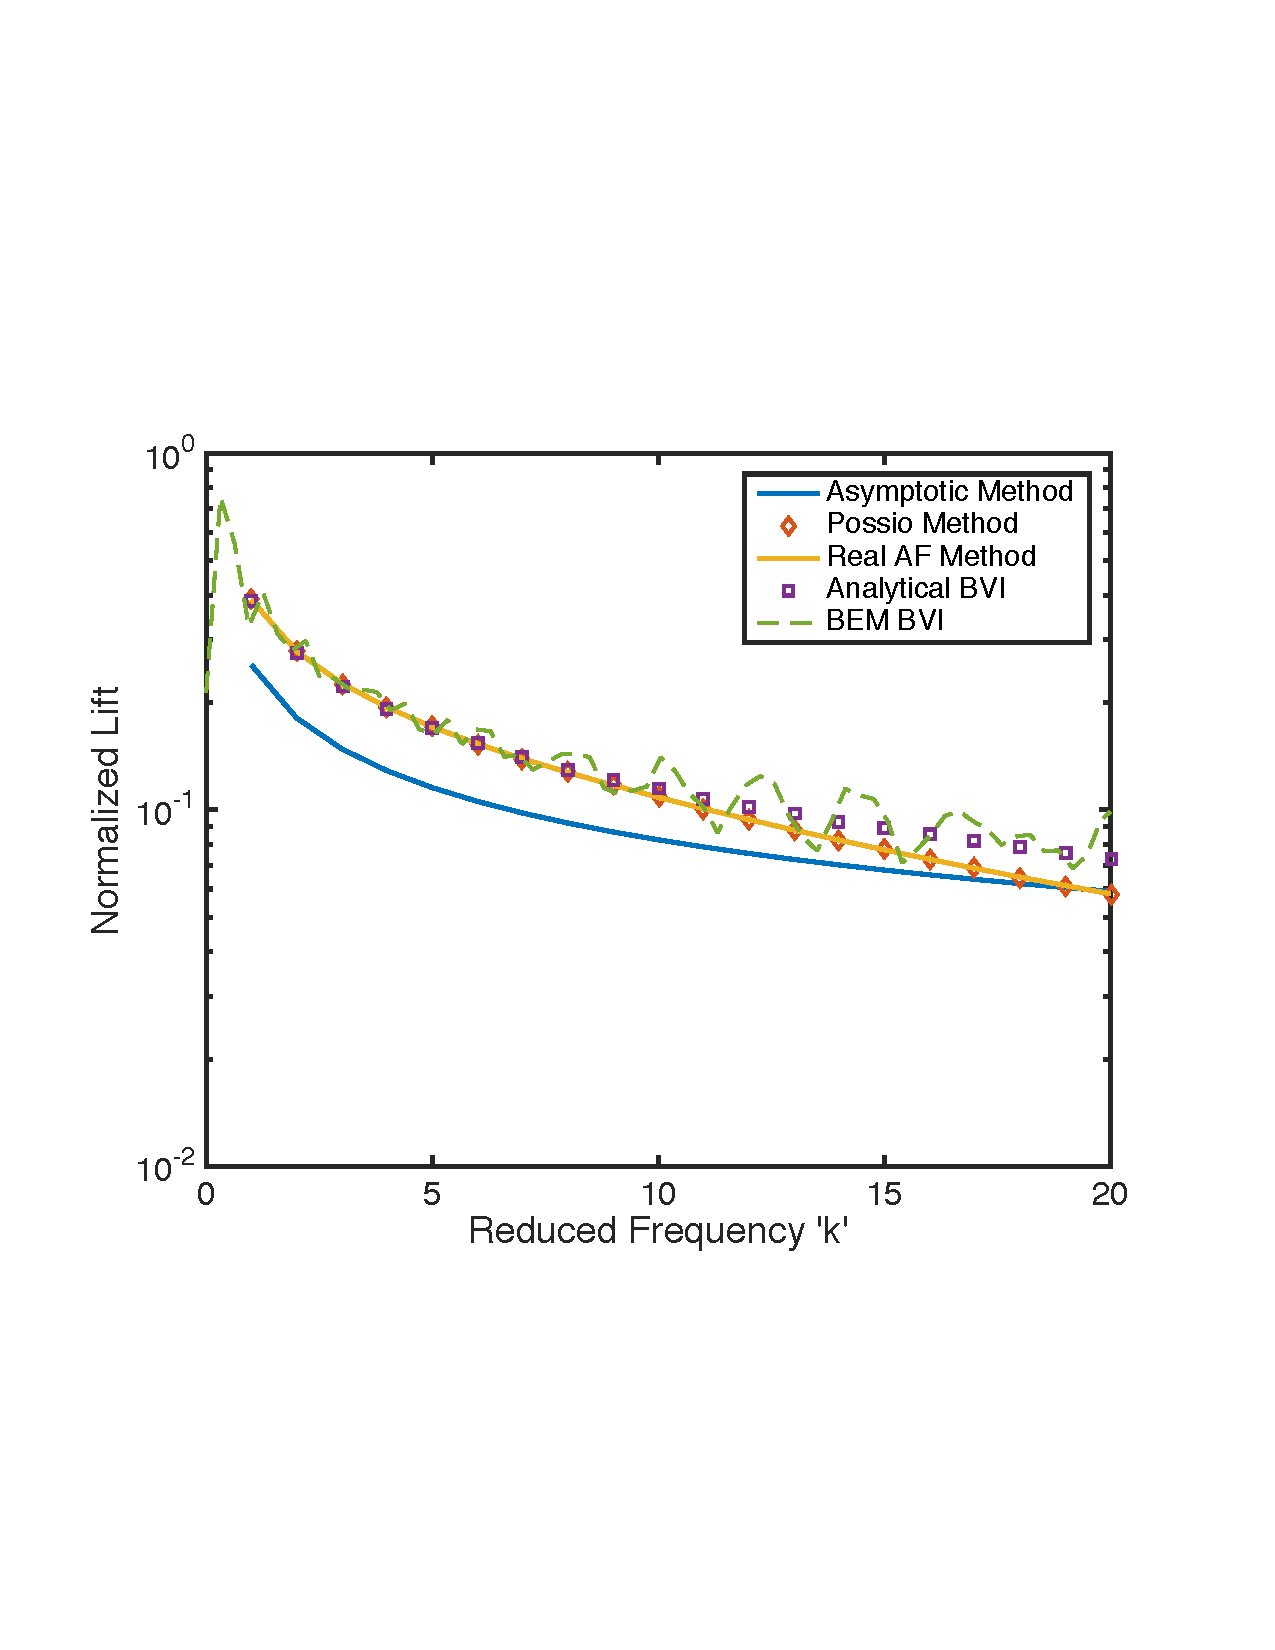
\includegraphics[width = 3.6 in, height = 2.5 in]{fp_total_compare}
\centering
\caption{Comparison of Lift Spectrums}
\end{figure}
\newpage
\noindent \textbf{Unsteady Pressure Distribution}\\ \\
\noindent Now, the pressure on the surface of the blade produced by the BEM code was also compared to the other simulations previously mentioned. The figures below show the magnitude, real and imaginary pressures on the surface of the airfoil. Several frequencies were selected for comparison from k=5 to k=20. The results were obtained by saving the pressure along the airfoil in time and then performing a fft on each point along the chord to produce a spectral analysis of the pressure. Certain reduced frequencies were selected and graphs of pressure vs. chord position were created for each reduced frequency of interest. \newline



\begin{figure}[h]
\centering
\begin{subfigure}{0.3\textwidth}
	\centering
	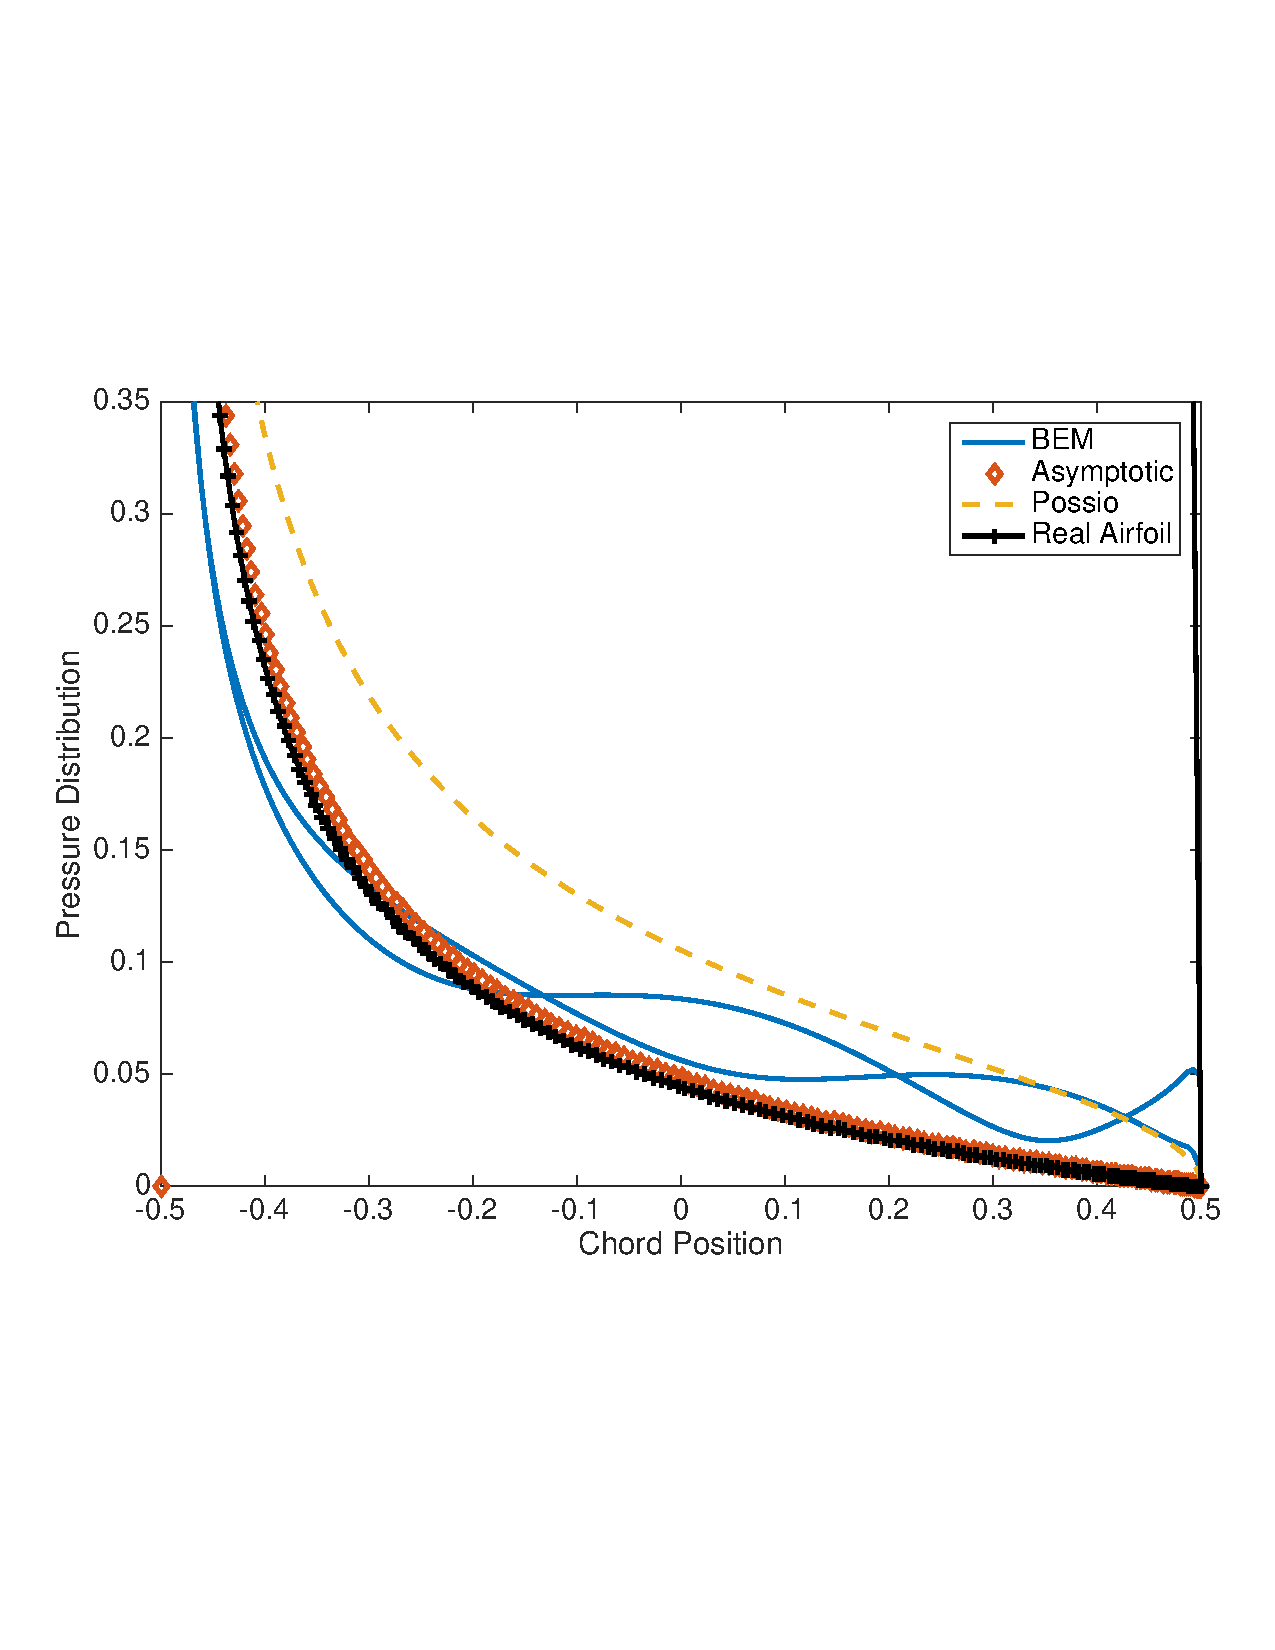
\includegraphics[width = \textwidth, height=0.2\textheight]{Pressure_k5}
	\captionof{figure}{Magnitude}
\end{subfigure}%
\begin{subfigure}{0.3\textwidth}
	\centering
	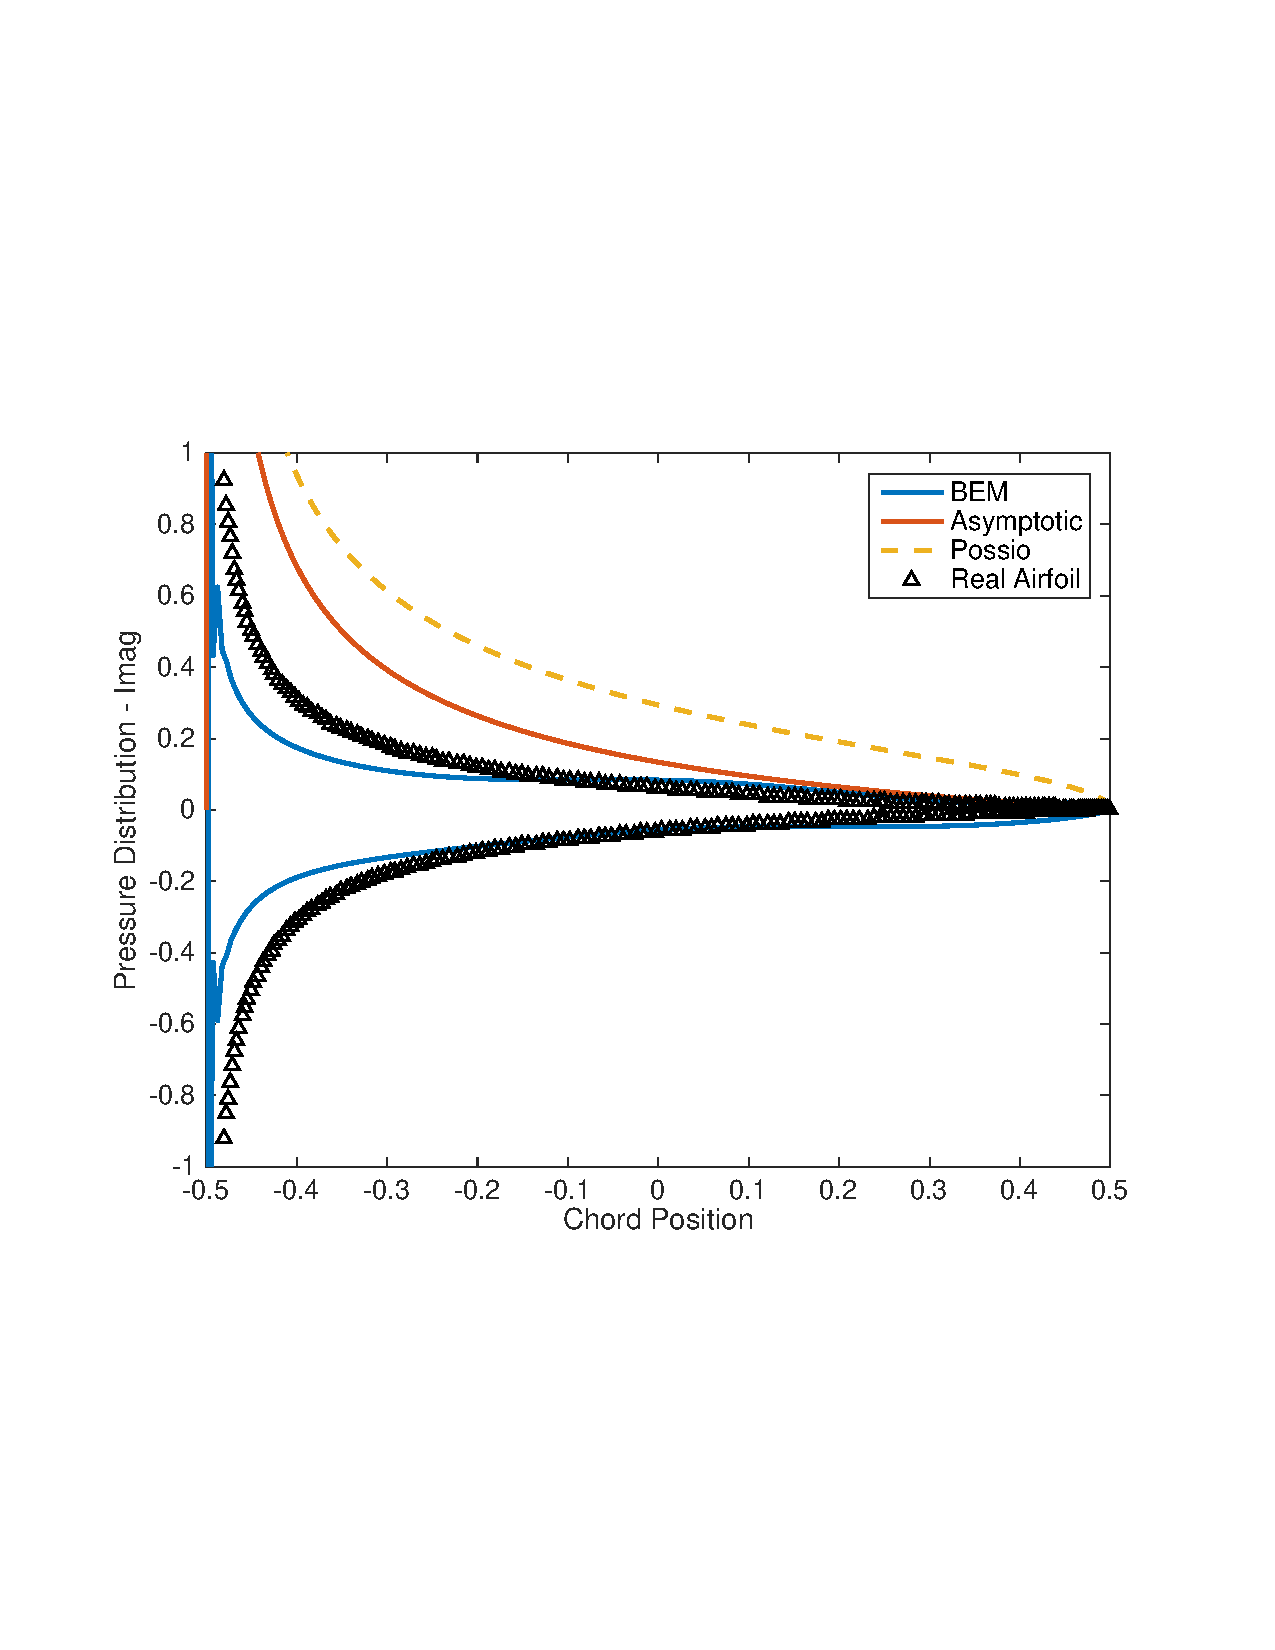
\includegraphics[width = \textwidth, height=0.2\textheight]{Pressure_k5imag}
	\captionof{figure}{Imaginary}
\end{subfigure}%
\begin{subfigure}{0.33\textwidth}
	\centering
	\includegraphics[width = \textwidth, height=0.2\textheight]{Pressure_k5real}
	\captionof{figure}{Real}
\end{subfigure}%
\caption{Pressure Distribution for a reduced frequency of k=5}
\end{figure}

\begin{figure}[h]
\centering
\begin{subfigure}{0.3\textwidth}
	\centering
	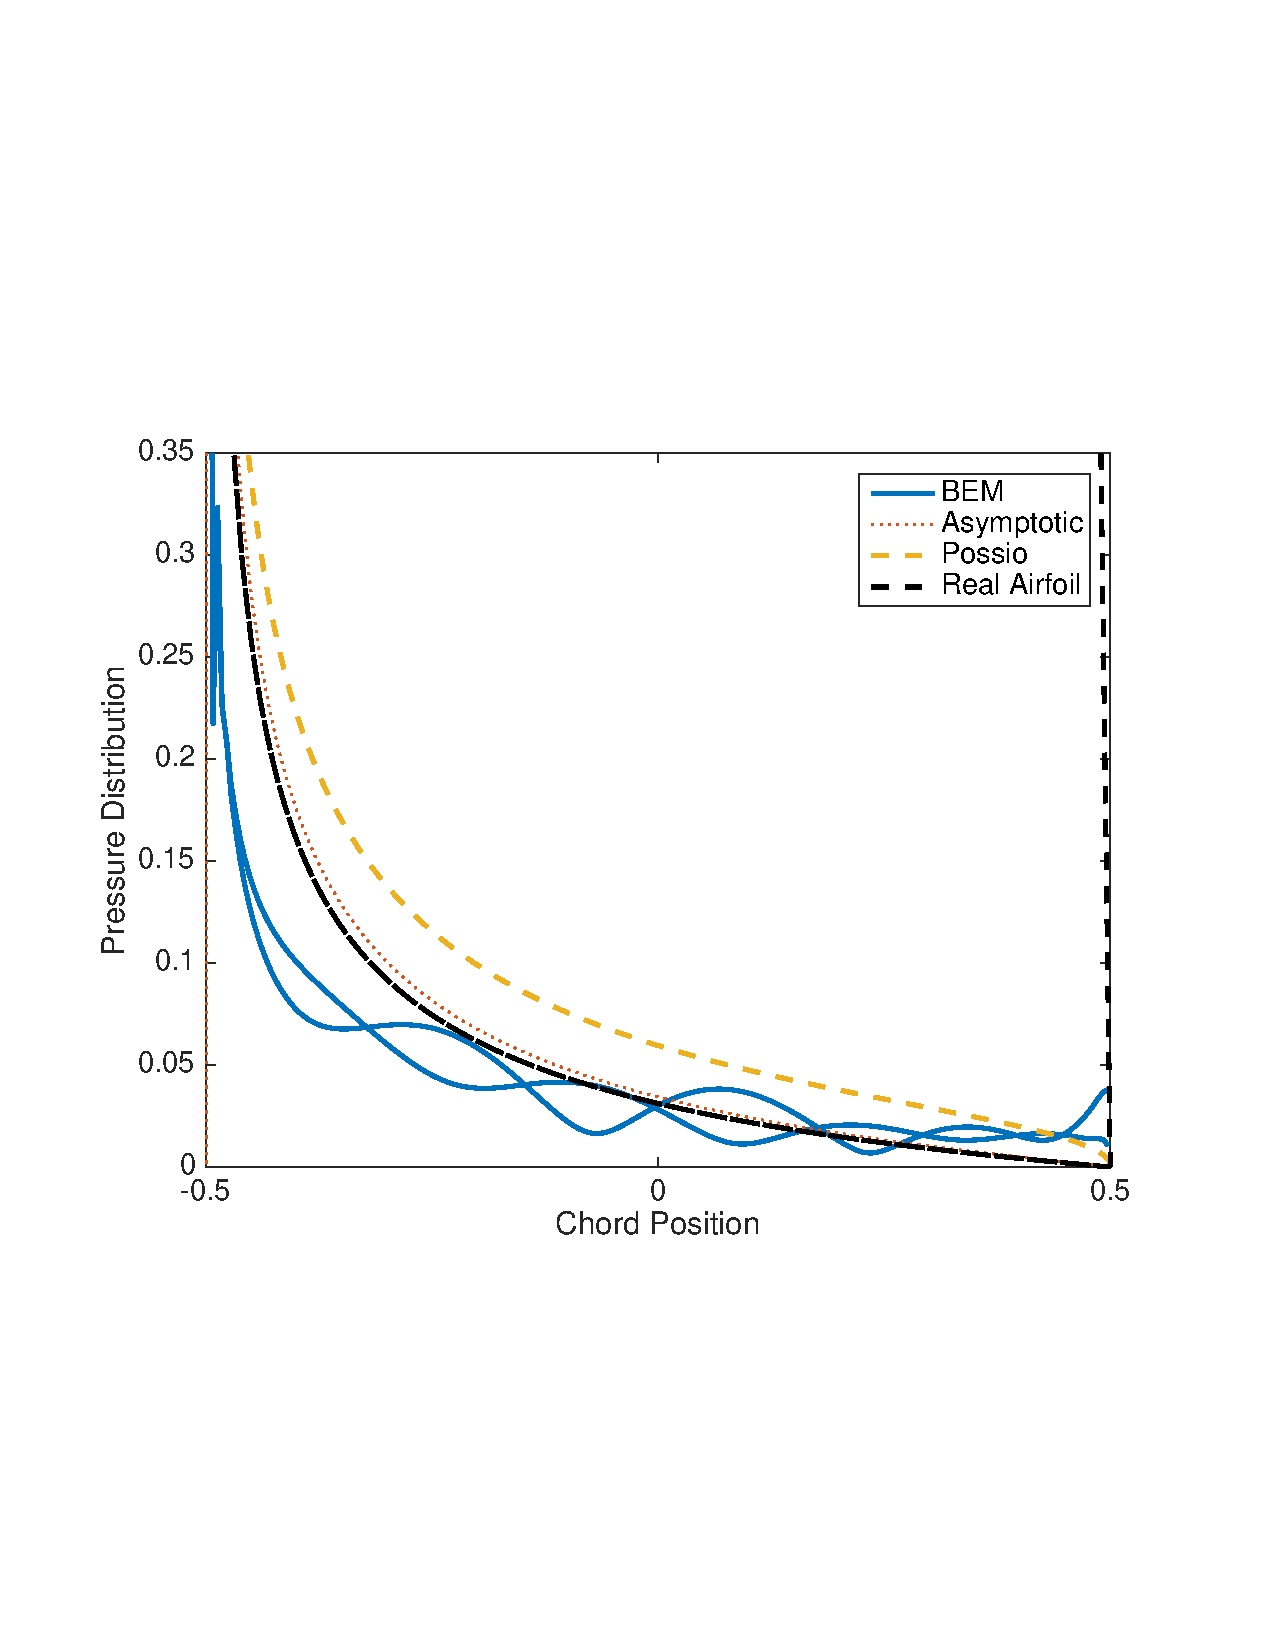
\includegraphics[width = \textwidth, height=0.2\textheight]{pressure_k10mag}
	\captionof{figure}{Magnitude}
\end{subfigure}%
\begin{subfigure}{0.3\textwidth}
	\centering
	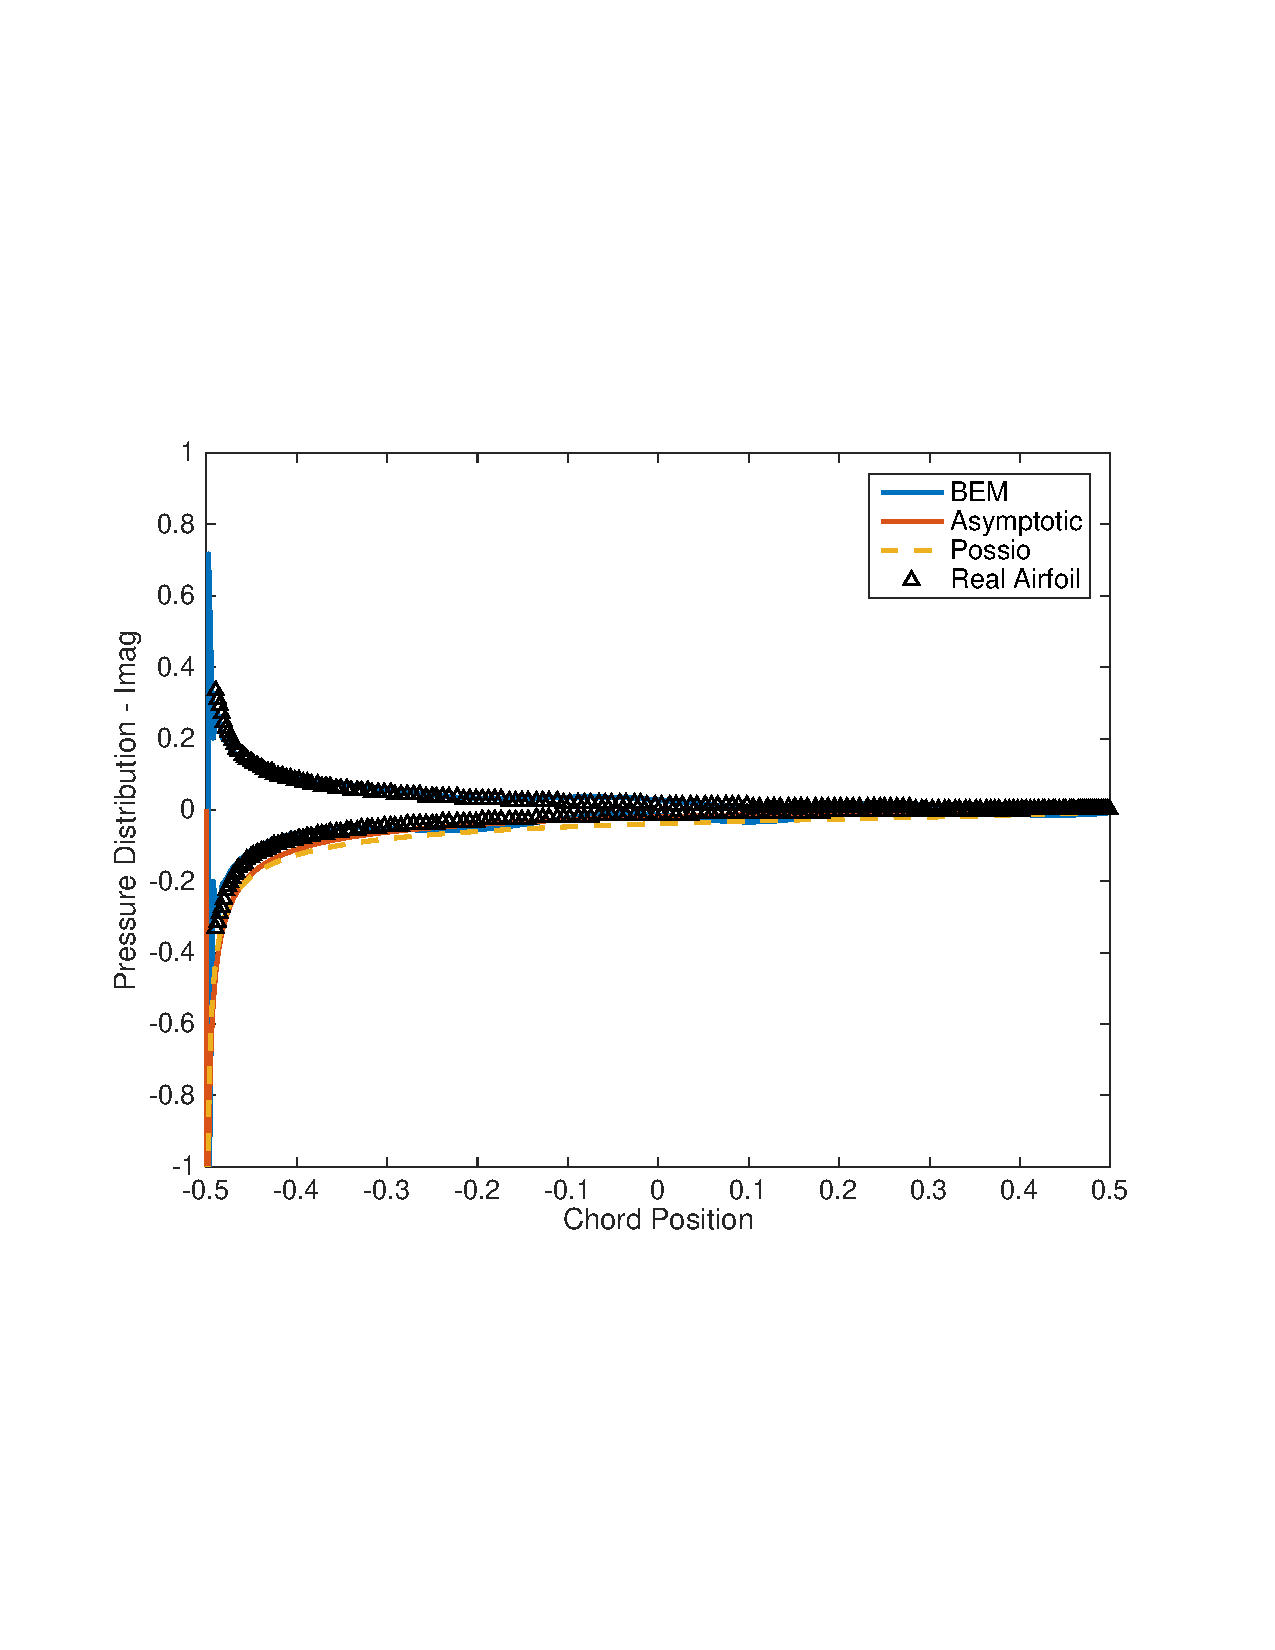
\includegraphics[width = \textwidth, height=0.2\textheight]{pressure_k10imag}
	\captionof{figure}{Imaginary}
\end{subfigure}%
\begin{subfigure}{0.33\textwidth}
	\centering
	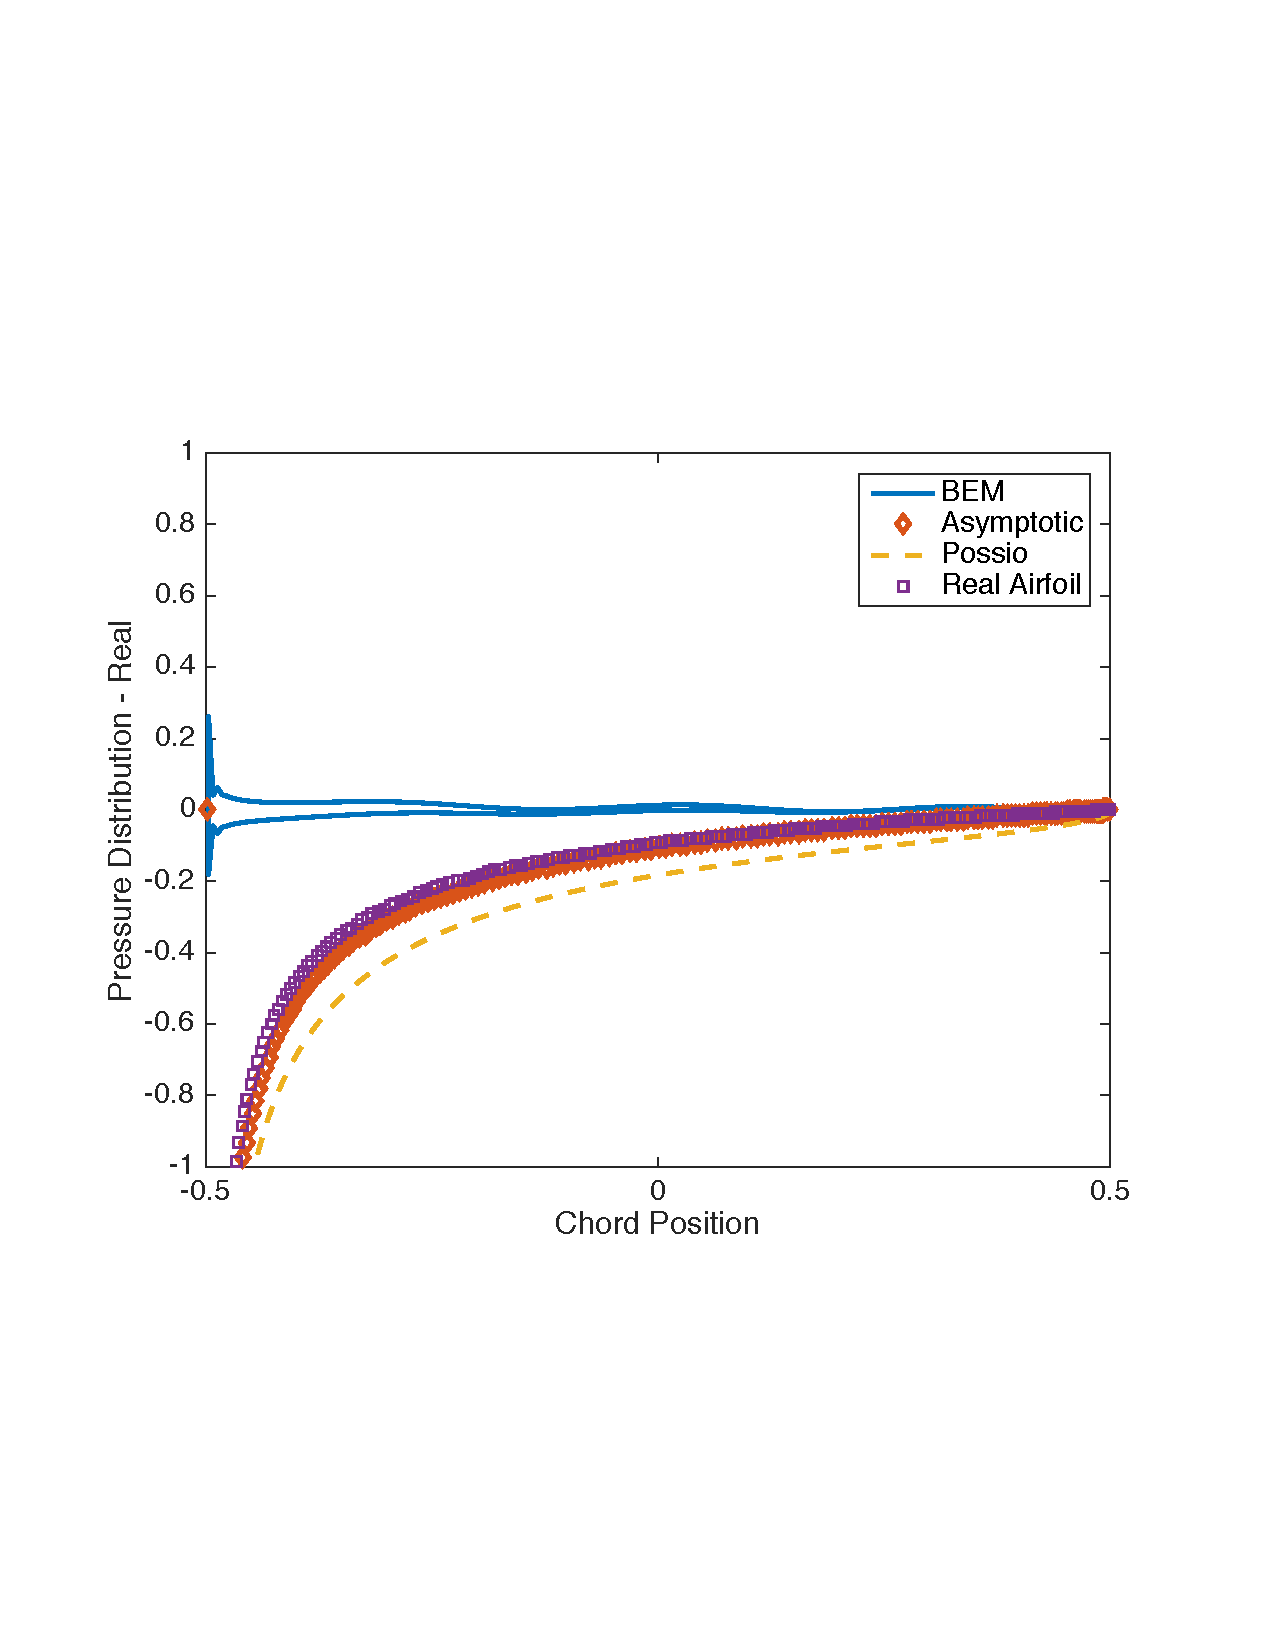
\includegraphics[width = \textwidth, height=0.2\textheight]{pressure_k10real}
	\captionof{figure}{Real}
\end{subfigure}%
\caption{Pressure Distribution for a reduced frequency of k=10}
\end{figure}

\newpage
\begin{figure}[h]
\centering
\begin{subfigure}{0.3\textwidth}
	\centering
	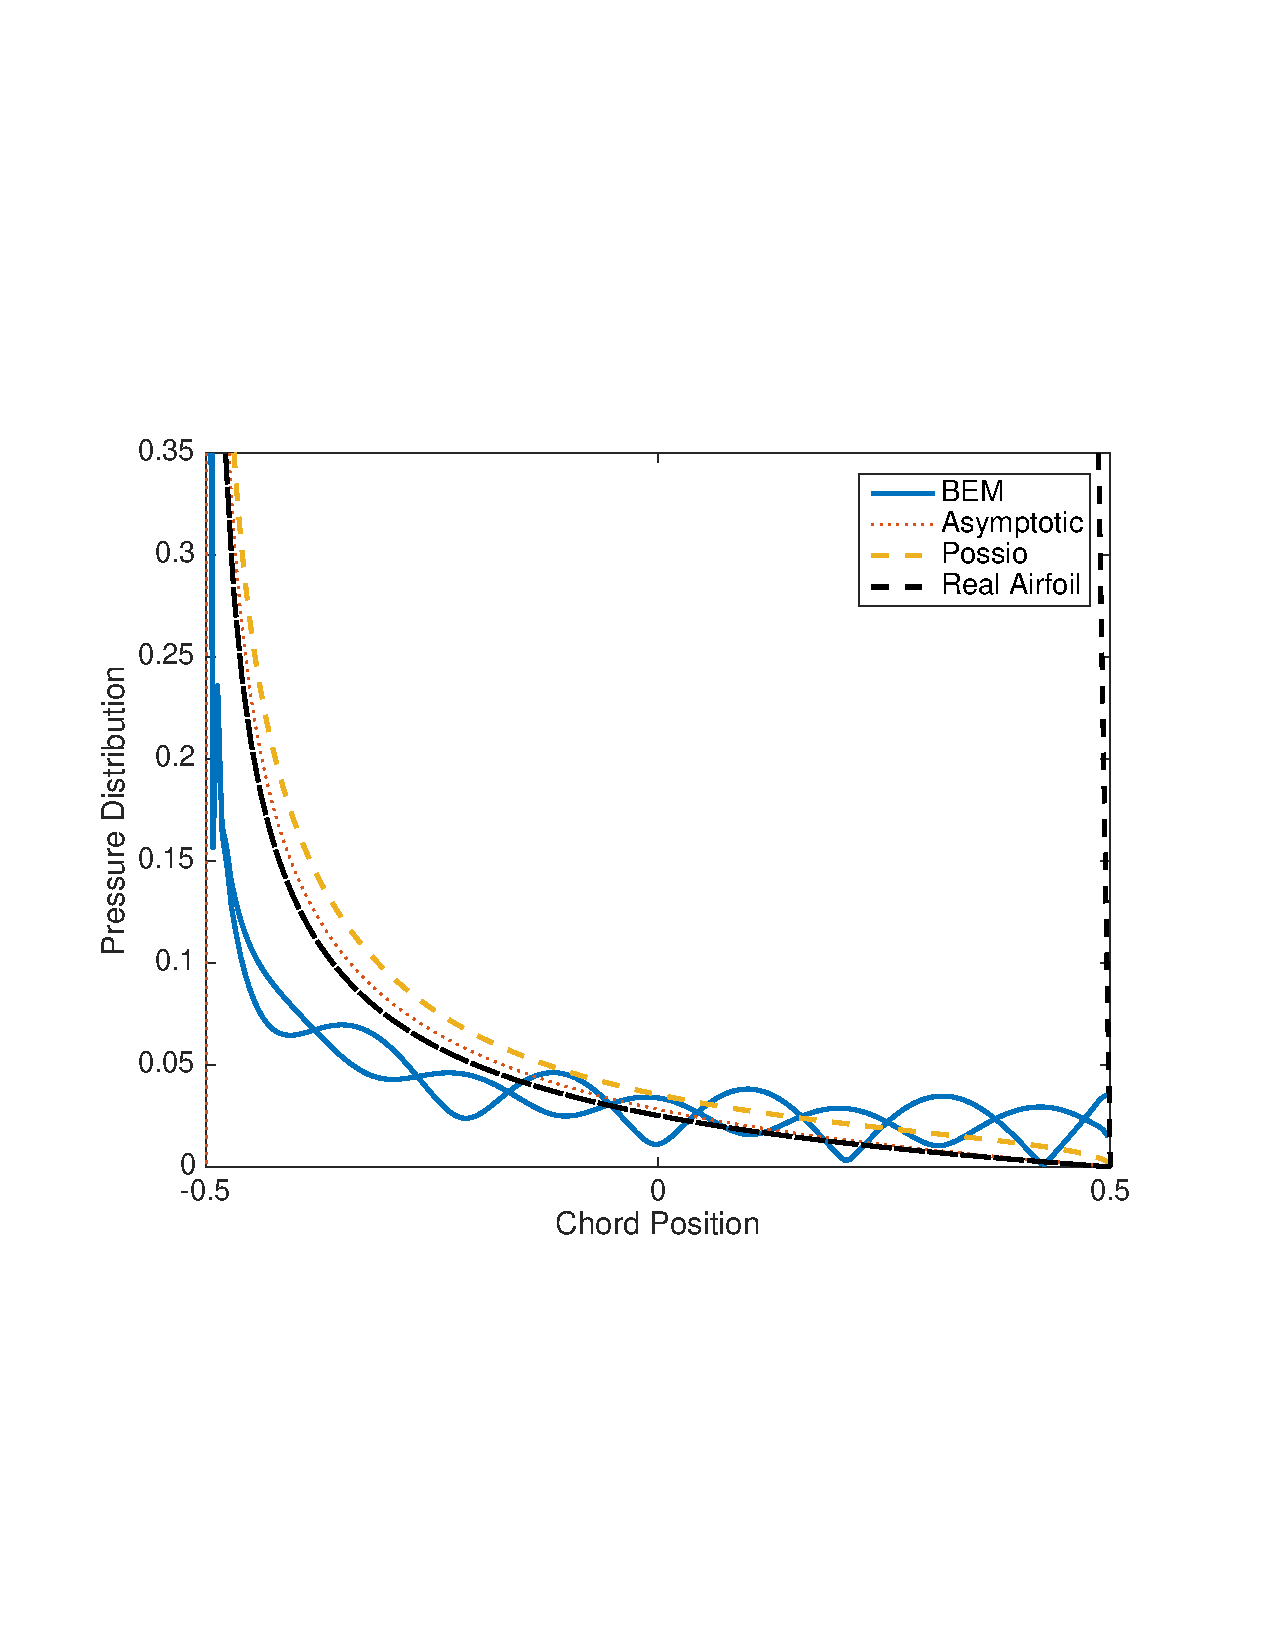
\includegraphics[width = \textwidth, height=0.2\textheight]{pressure_k15mag}
	\captionof{figure}{Magnitude}
\end{subfigure}%
\begin{subfigure}{0.3\textwidth}
	\centering
	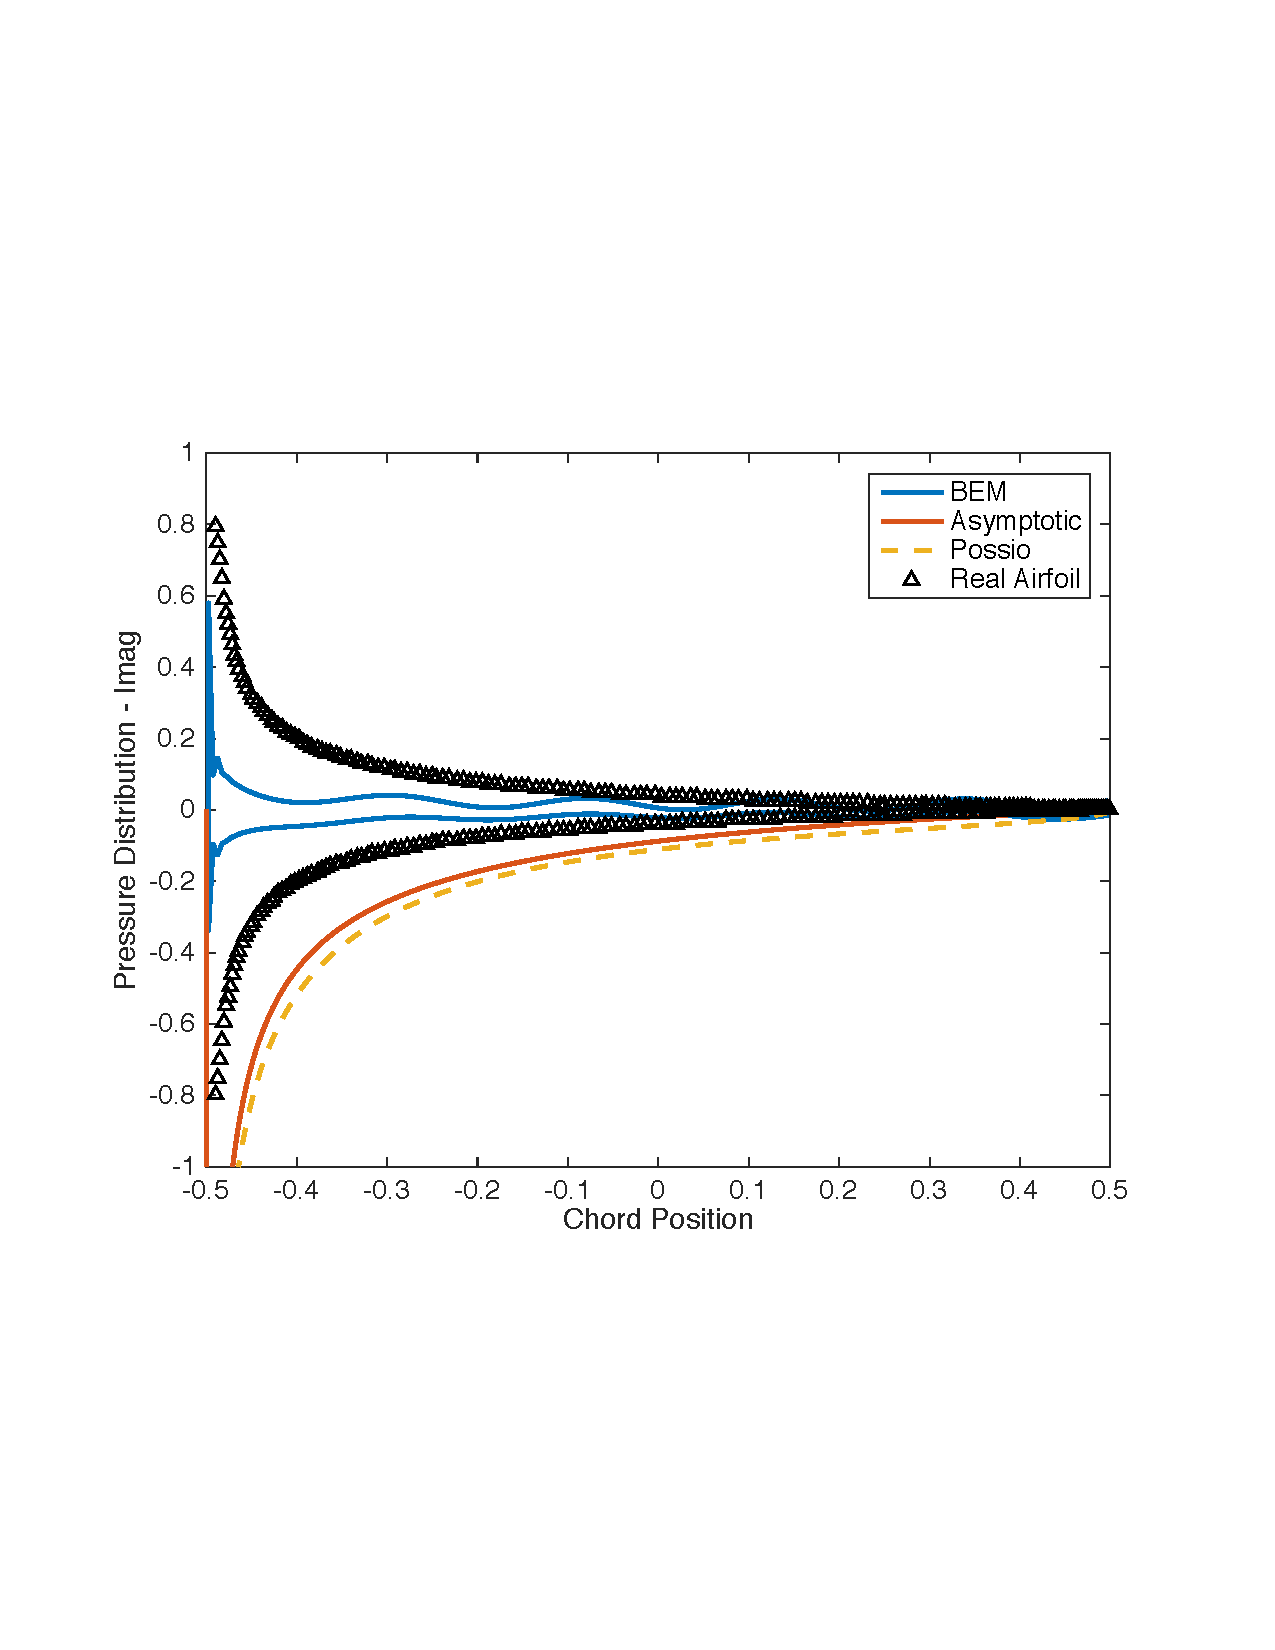
\includegraphics[width = \textwidth, height=0.2\textheight]{pressure_k15imag}
	\captionof{figure}{Imaginary}
\end{subfigure}%
\begin{subfigure}{0.33\textwidth}
	\centering
	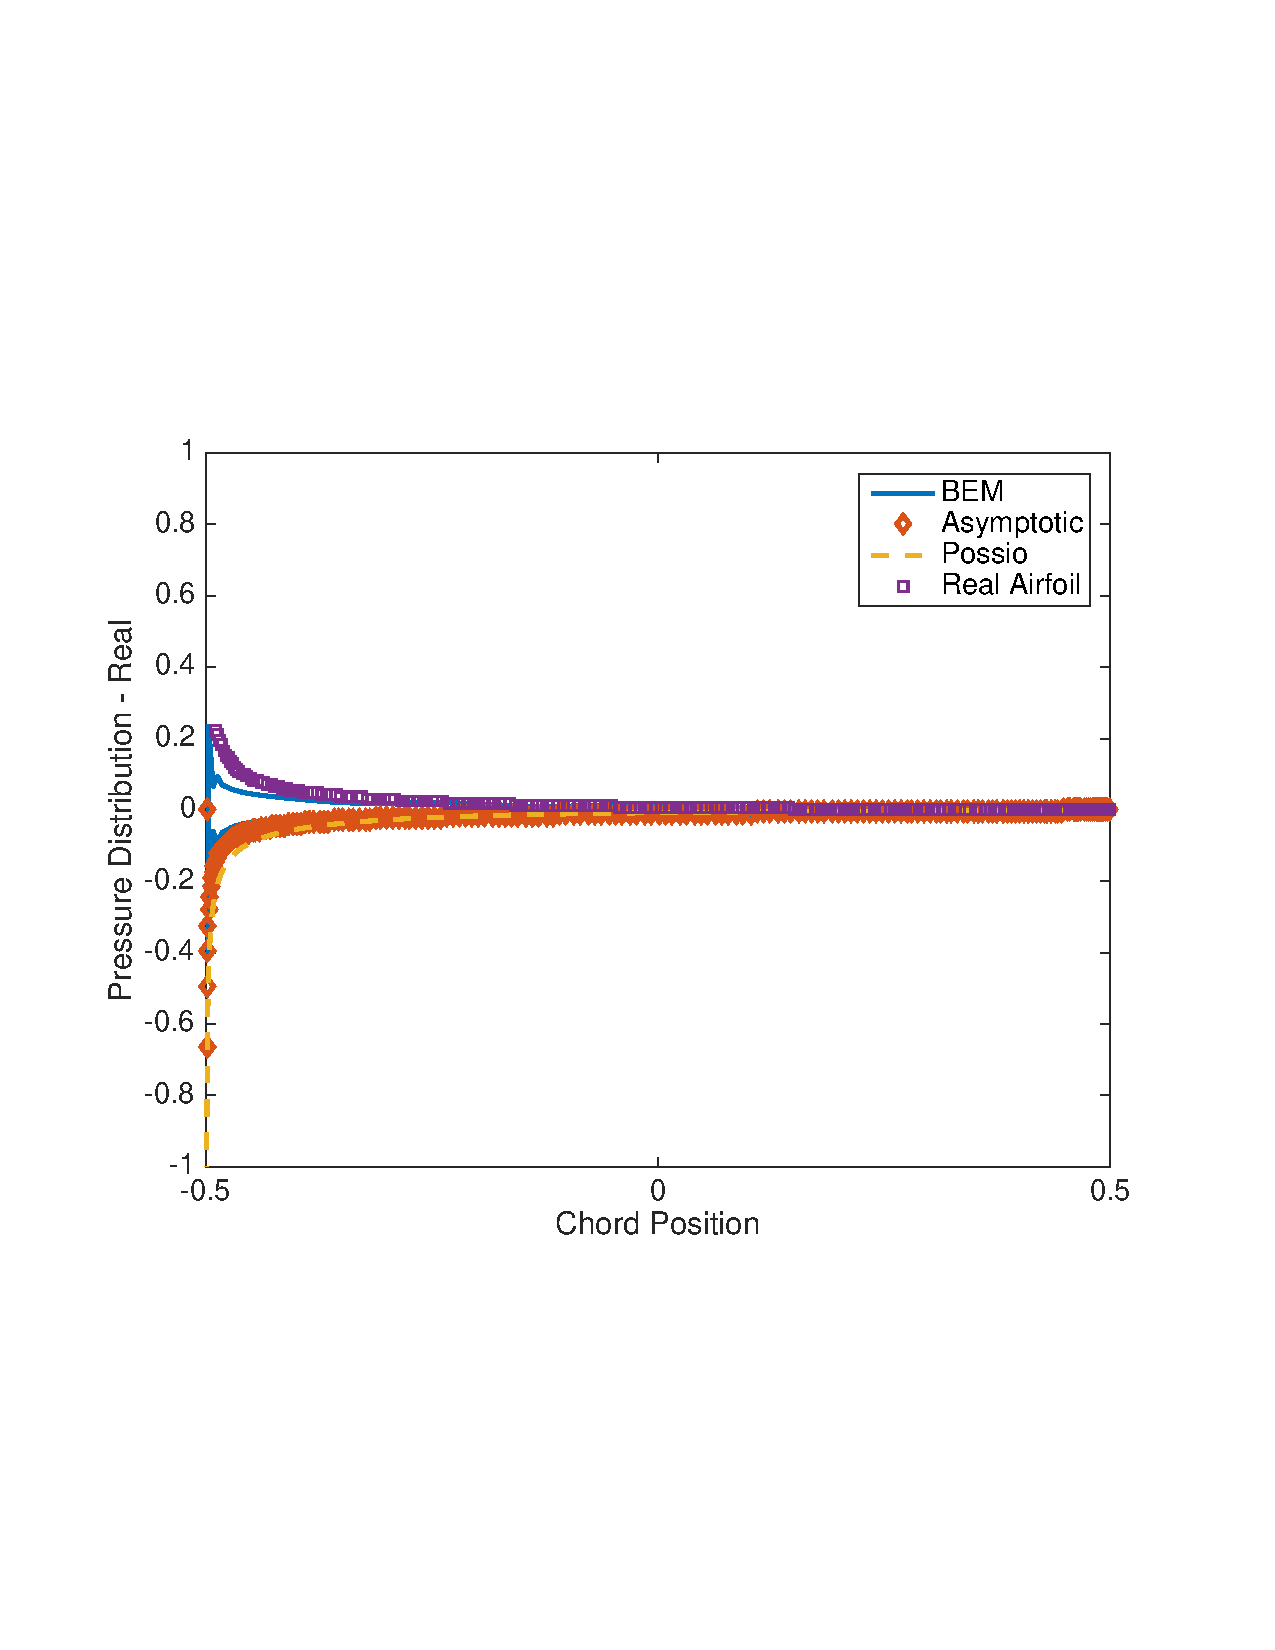
\includegraphics[width = \textwidth, height=0.2\textheight]{pressure_k15real}
	\captionof{figure}{Real}
\end{subfigure}%
\caption{Pressure Distribution for a reduced frequency of k=15}
\end{figure}

\begin{figure}[h]
\centering
\begin{subfigure}{0.3\textwidth}
	\centering
	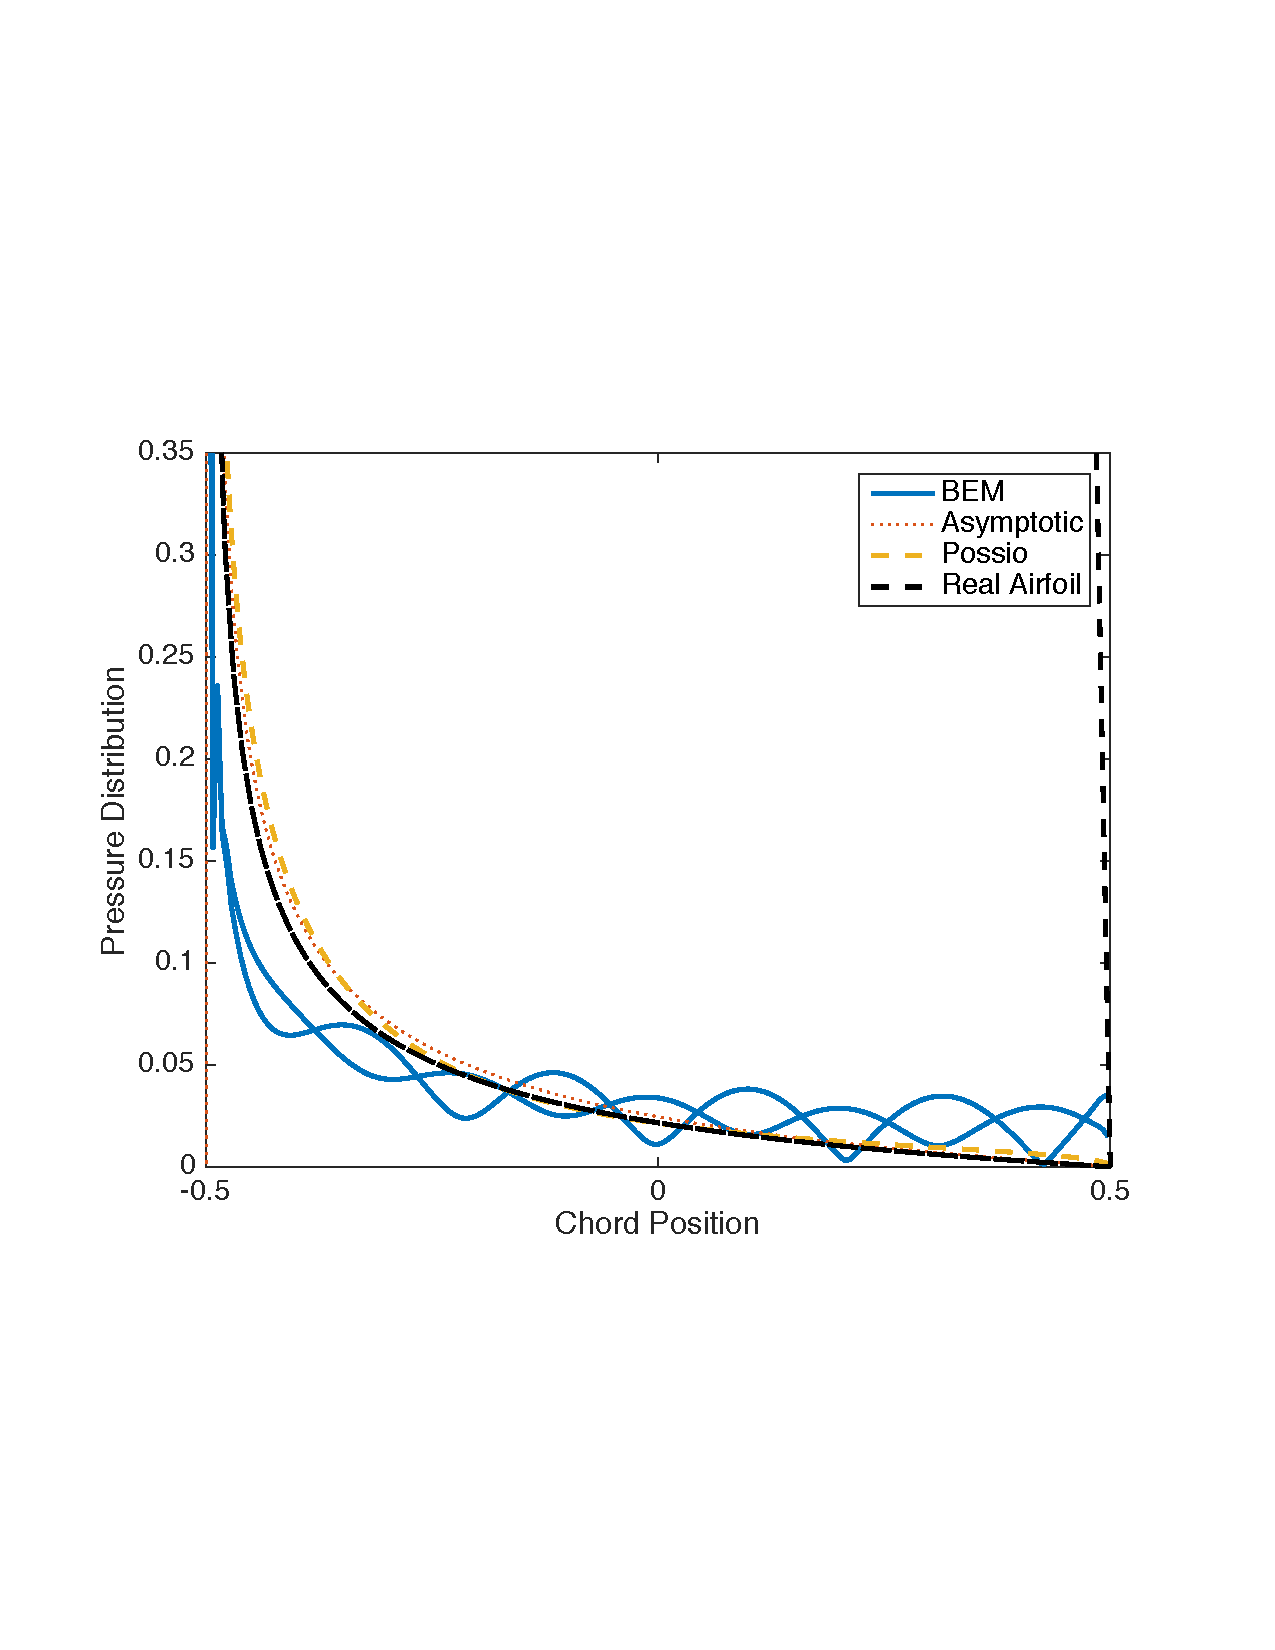
\includegraphics[width = \textwidth, height=0.2\textheight]{pressure_k20mag}
	\captionof{figure}{Magnitude}
\end{subfigure}%
\begin{subfigure}{0.3\textwidth}
	\centering
	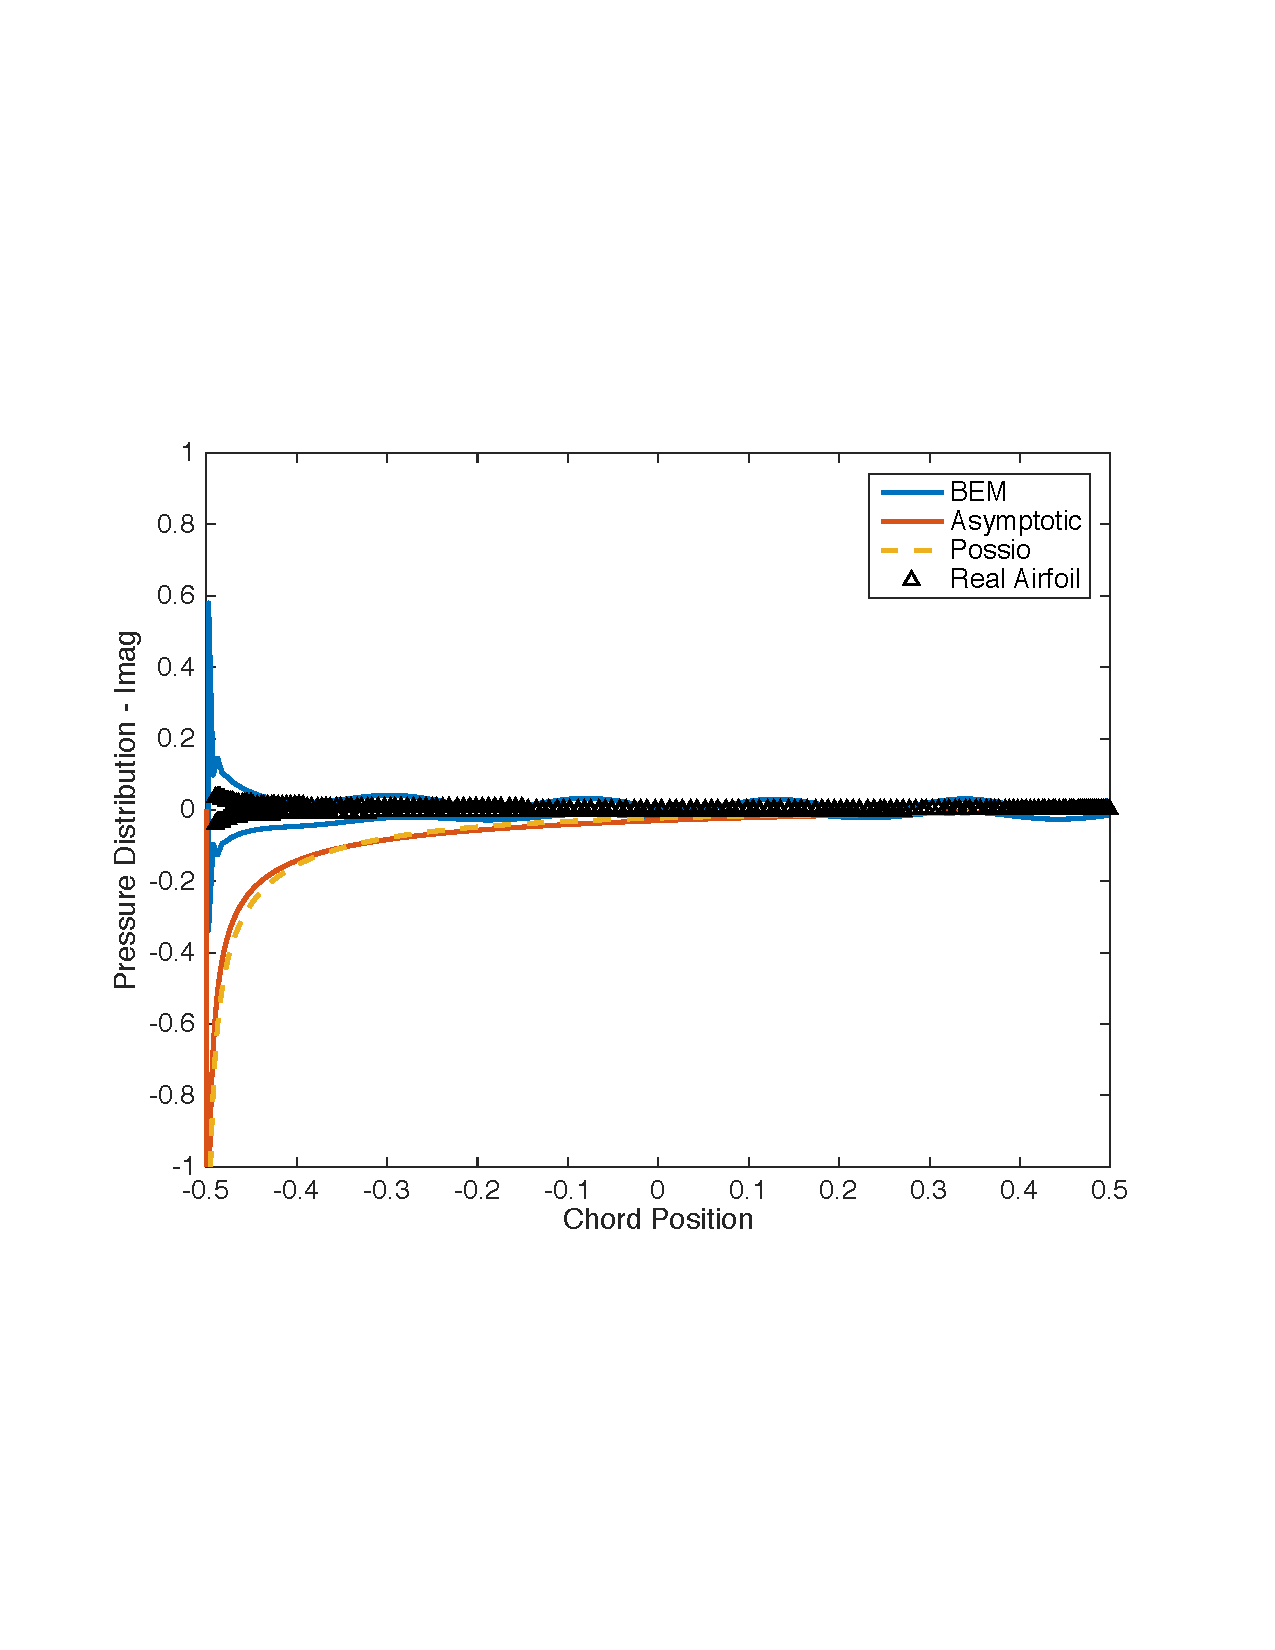
\includegraphics[width = \textwidth, height=0.2\textheight]{pressure_k20imag}
	\captionof{figure}{Imaginary}
\end{subfigure}%
\begin{subfigure}{0.33\textwidth}
	\centering
	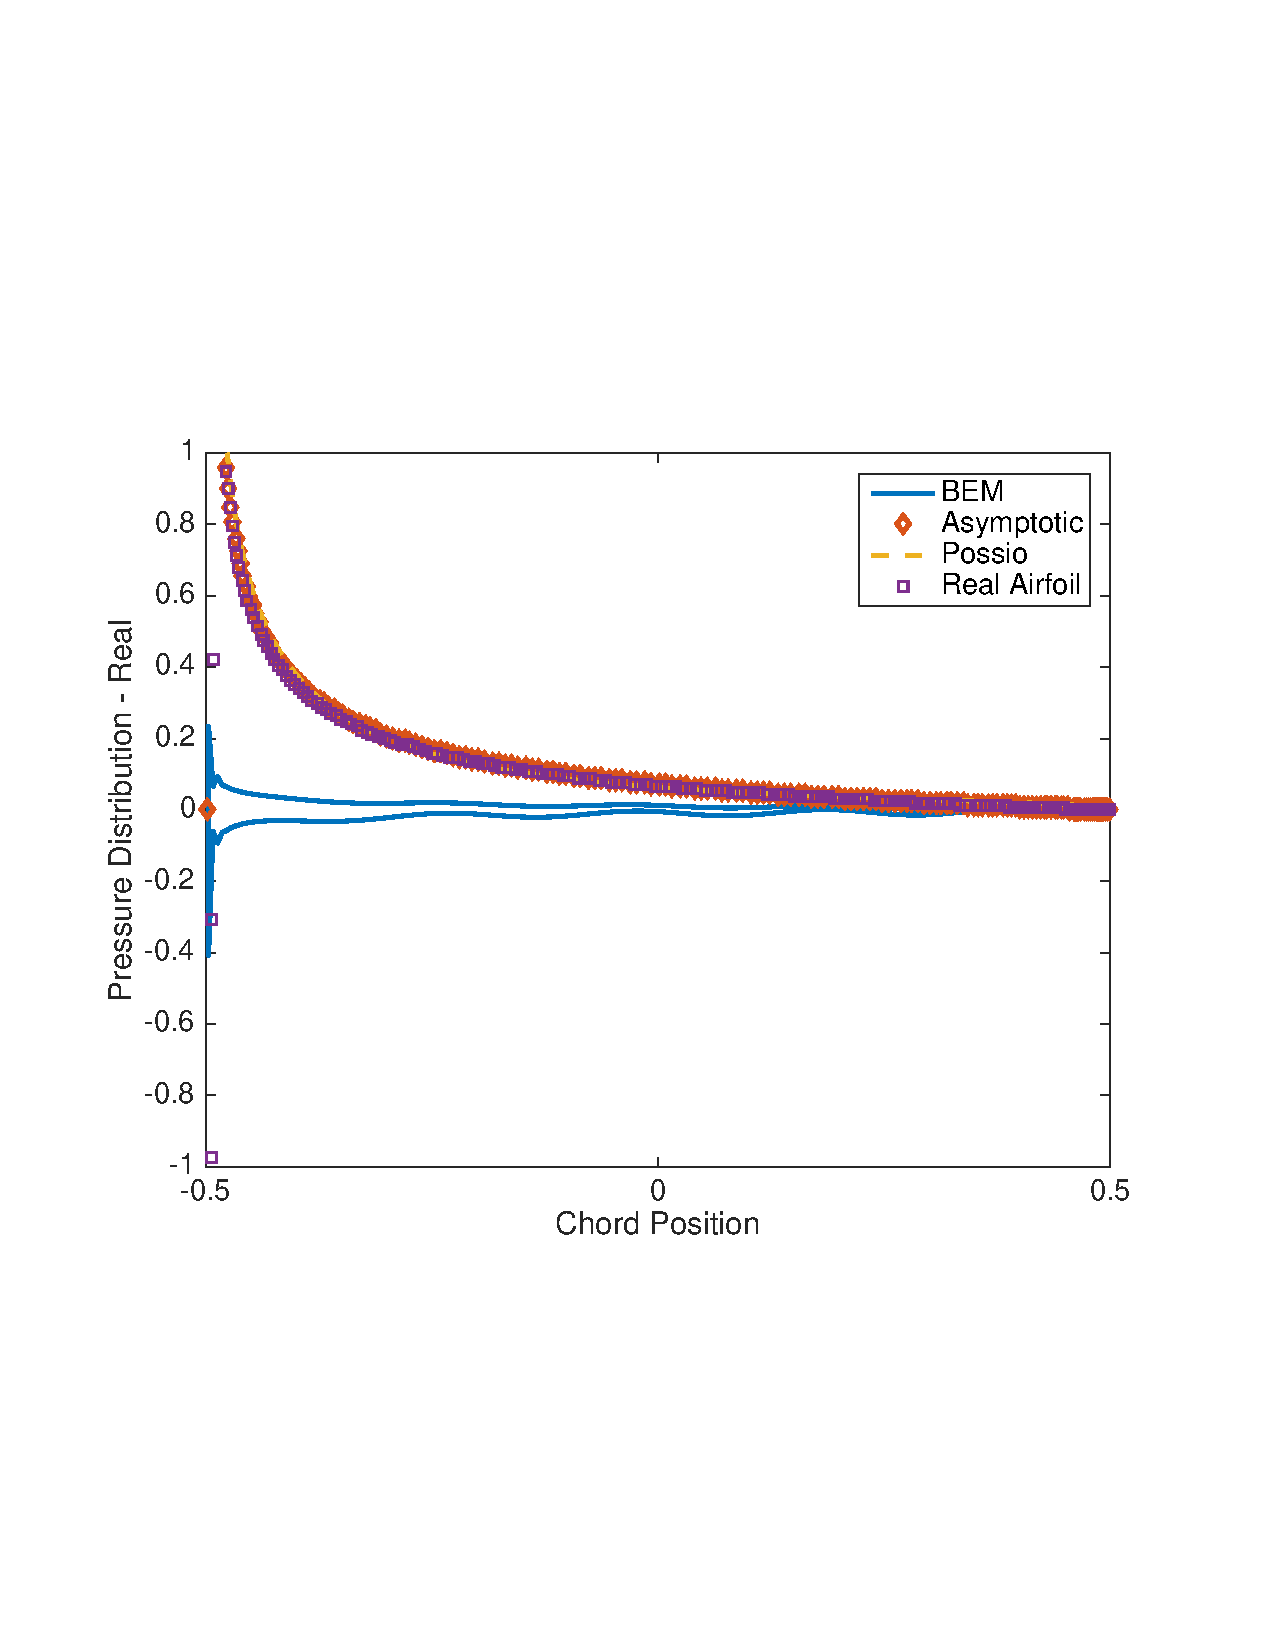
\includegraphics[width = \textwidth, height=0.2\textheight]{pressure_k20real}
	\captionof{figure}{Real}
\end{subfigure}%
\caption{Pressure Distribution for a reduced frequency of k=20}
\end{figure}




\end{document}


